\chapter{Background}
\label{chap:background}

\section{Preliminaries: Model and Correctness}
\label{sec:prelims}
\chapter{Preliminaries}
\label{chap:prelims}

We consider a shared memory model, where a finite number of threads execute \emph{operations} on shared \emph{objects}. An operation consists of an \emph{invocation} and a matching \emph{response}. A \emph{history} \(\mathnormal{H}\) is a finite sequence of operation invocation and response steps. A history \(\mathnormal{H}\) defines a partial order \(\prec_\mathnormal{H}\) on operations: Given operations \(op\) and \(op'\), \(op \prec_H op'\) if and only if \(response(op)\) precedes \(invocation(op')\) in \(\mathnormal{H}\). Two operations that do not precede each other are \emph{concurrent}. In a \emph{sequential history}, there are no concurrent operations. An object is specified using a \emph{sequential specification} $\mathcal{H}$, which is the set of its allowed sequential histories.
An operation \emph{op} is \emph{complete} in a history \(\mathnormal{H}\) if both \(invocation(op)\) and its matching \(response(op)\) are in \(\mathnormal{H}\).
A \emph{linearization} of a concurrent history \(\mathnormal{H}\), is a sequential history $H'$ such that: (1) $H' \in \mathcal{H}$, (2) $H'$ contains all completed operations and possibly additional non-complete ones, after adding matching responses, and, (3) $\prec_{H'}$ extends $\prec_H$. A correctness condition for randomized algorithms \emph{strong linearizability}~\cite{strong_linearizability}, defined as follows: 

\begin{definition}[strong linearizability]
\label{def:strong_linearizability}
A function \(f\) mapping executions to histories is \emph{prefix-preserving} if for any two executions $\sigma$, $\sigma$', where $\sigma$ is a prefix of $\sigma$', $f(\sigma)$ is a prefix of $f(\sigma')$. 
An object A is \emph{strongly linearizable} if there is a prefix-preserving function \(f\) that maps every history \(\mathnormal{H}\) of $A$ to a linearization of \(\mathnormal{H}\).
\end{definition}

Our algorithm is randomised and we consider a weak adversary that determines the scheduling without observing the coin-flips.

As previously mentioned, we adopt a flavor of \emph{relaxed semantics}, as defined in \cite{Henzinger_2013_Quantitative_Relaxation}:

\begin{definition}[$r$-relaxation] \label{def:r-relaxtion}
A sequential history $H$ is an \emph{$r$-relaxation} of a sequential history H', if H is comprised of all but at most $r$ of the invocations in $H'$ and their responses,
and each invocation in $H$ is preceded by all but at most $r$ of the invocations that precede the same invocation in $H'$.
The $r$-relaxation of a sequential specification $\mathcal{H}$ is the set of histories that have $r$-relaxations in $\mathcal{H}$:
\[{H}^r \triangleq \left\{ H' \mid \exists H \in \mathcal{H}: H \text{ is an } r\text{-relaxation of } H'\right\}. \]
\end{definition}


\section{Problem Definition} \label{sec:problem_define}

Given a stream $A=x_1,x_2,\dots,x_n$ with $n$ elements,
the \emph{rank} of some $x$ (not necessarily in $A$) is the number of elements smaller than $x$ in $A$, denoted \gls{Rank}. For any $0 \leq \phi \leq 1$, the \emph{$\phi$ quantile} of $A$ is an element $x$ such that $R(A,x)=\lfloor \phi n \rfloor$.

A Quantiles sketch's \gls{API} is as follows:
\begin{itemize}
\item \textbf{update(}$x$\textbf{)} process stream element $x$;
\item \textbf{query(}$\phi$\textbf{)} return an approximation of the $\phi$ quantile in the stream processed so far. 
\end{itemize}
A PAC Quantiles sketch with parameters \gls{epsilon}, \gls{delta} returns element $x$ for query($\phi$) after n updates such that $R(A,x) \in \left[ (\phi-\epsilon)n,(\phi+\epsilon)n  \right]$, with probability at least $1-\delta$.

In an $r$-relaxed sketch for some $r\geq0$ every query returns an estimate of the $\phi$ quantile in a subset of the stream processed so far including all but at most $r$ stream elements~\cite{Henzinger_2013_Quantitative_Relaxation, Rinberg_2020_fast_sketches}.


\section{Sequential Implementation} \label{sec:seq_imp}


The Quantiles sketch proposed by Agarwal et al.~\cite{mergeables_summaries} consists of a hierarchy of arrays, where each array summarizes a subset of the overall stream. The sketch is instantiated with a parameter \gls{k}, which is a function of $(\epsilon,\delta)$. The first array, denoted level $0$, consists of at most $2k$ elements, and every subsequent array, in levels $1,2,\dots$, consists of either $0$ or $k$ elements at any given time.

Stream elements are processed in order of arrival, first entering level $0$, until it consists of $2k$ elements. Once this level is full, the sketch samples the array by sorting it and then selecting either the odd indices or the even ones with equal probability. The $k$ sampled elements are then propagated to the next level, and the rest are discarded. If the next level is full, i.e., consists of $k$ elements, then the sketch samples the union of both arrays by performing a merge sort, and once again retaining either the odd or even indices with equal probability. This propagation is repeated until an empty level is reached. Every level that is sampled during the propagation is emptied. Figure~\ref{fig: quantiles_sketch} depicts the processing of $4k$ elements.

\begin{figure}[h]
    \centering
    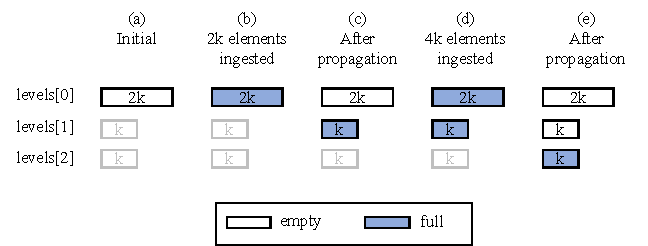
\includegraphics[width=\columnwidth]{graphics/sequential/seq_propagation.pdf}
    \caption{Quantiles sketch structure and propagation.}
    \label{fig: quantiles_sketch}
\end{figure}


Each element is associated with a \emph{weight}, which is the number of coin flips it has ``survived''. An element in an array on level $i$ has a weight of $2^i$, as it was sampled $i$ times. Thus, an element with a weight of $2^i$ represents $2^i$ elements in the processed stream.
For approximating the $\phi$ quantile, we construct a list of tuples, denoted \emph{samples}, containing all elements in the sketch and their associated weights. The list is then sorted by the elements' values. Denote by $W(x_i)$ the sum of weights up to element $x_i$ in the sorted list. The estimation of the $\phi$ quantile is an element $x_j$, such that $W(x_j) \leq \lfloor\phi n\rfloor$ and $W(x_{j+1}) > \lfloor\phi n\rfloor$.